\subsection{RWS}
\label{subsec:rws}

\paragraph{RWS}
\textbf{R}ange \textbf{W}hile \textbf{S}earch

\begin{itemize}
    \item \textbf{Fast, Long(er)-Range Search}
    \begin{itemize}
        \item radar scans selectable search volume
        \item displays raw target position returns
    \end{itemize}
    \item \textbf{No track data} 
    \begin{itemize}
        \item exact target range, velocity, angle, etc.
        \item but can transition to advanced modes
    \end{itemize}
    % (exact target range, velocity, angle, etc.)
    % --- but can transition to advanced modes
\end{itemize}

\begin{figure}[htbp]
    \centering
    \begin{tikzpicture}[auto, node distance=10mm, x=1mm, y=1mm, very thick, line cap=round,
        >={Latex[round]}
        ]
        
        \node[] (fig) at (0,0) {
            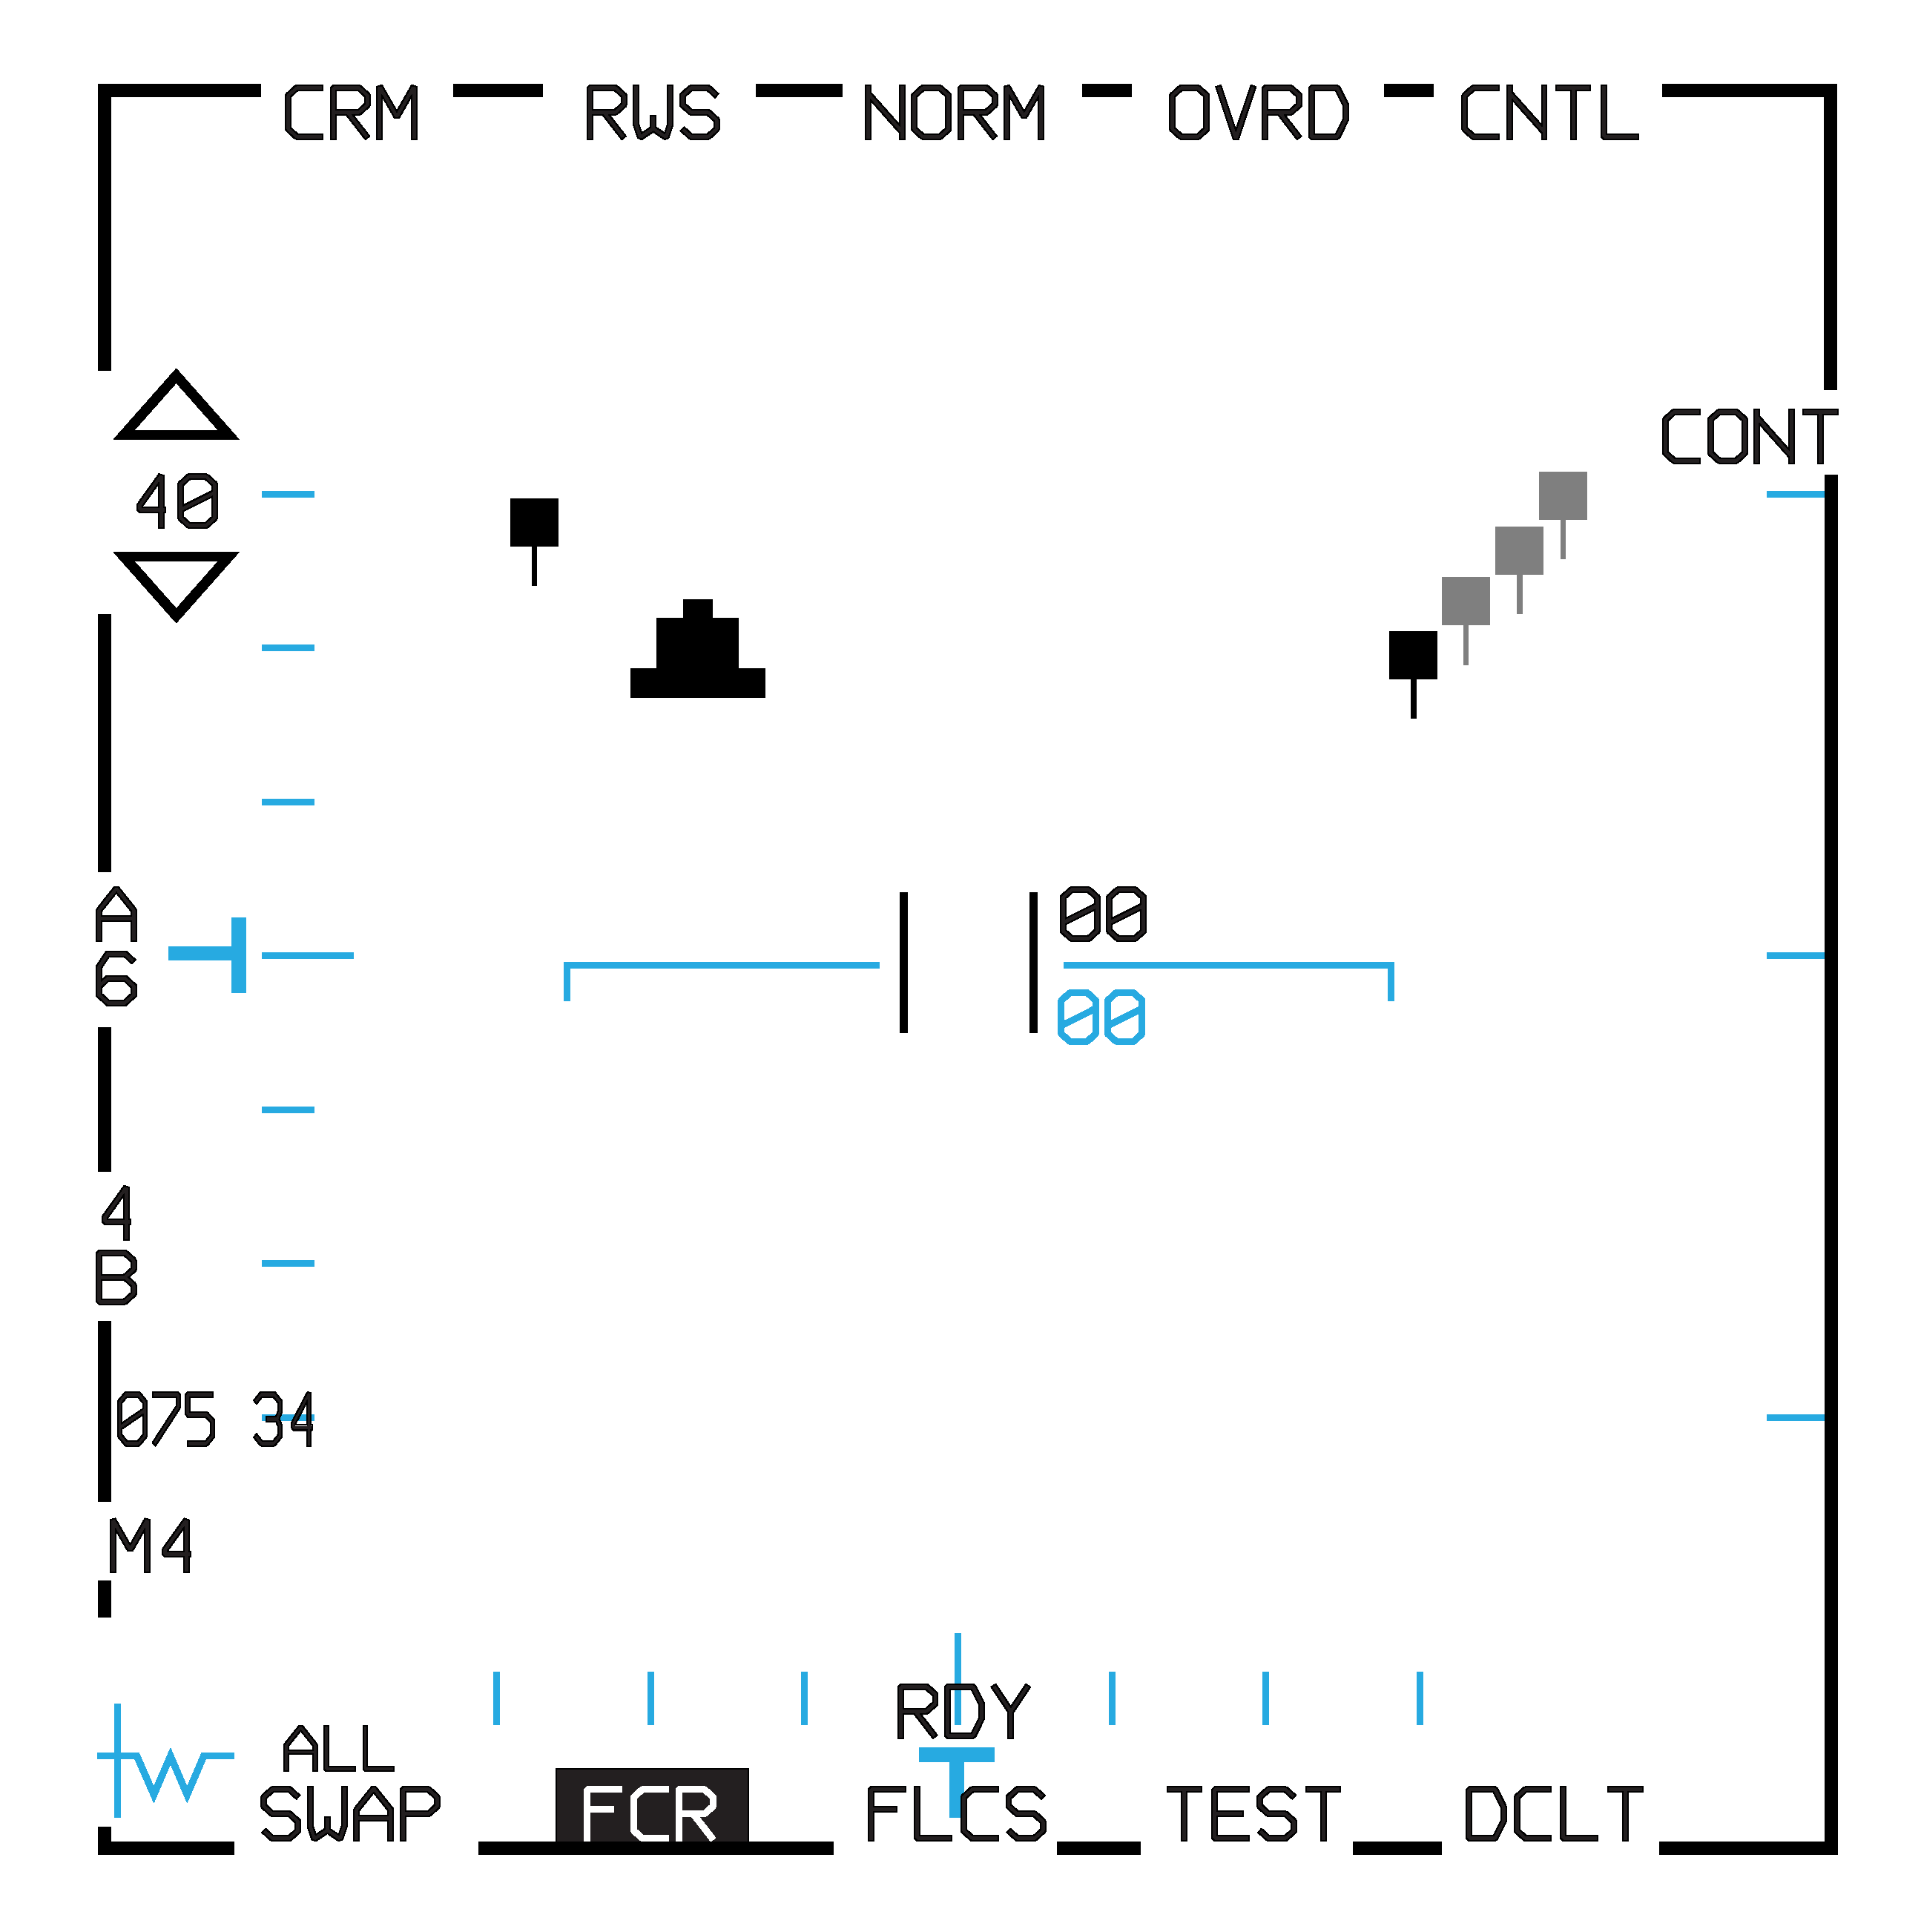
\includegraphics[
                height=75mm,
            ]{mfd/fcr_aa/rws_search.pdf}
        };

        % Annotations
        \node[lannot] (rsel) at ($(fig.west)+(0mm,18mm)$) {Range select};
        \draw[annotptr] (rsel.east) -- ++(4.5mm, 0mm);

        \node[lannot] (asel) at ($(fig.west)+(0mm,0.5mm)$) {Azimuth select};
        \draw[annotptr] (asel.east) -- ++(4.5mm, 0mm);

        \node[lannot] (bsel) at ($(fig.west)+(0mm,-10.5mm)$) {Elevation bar select};
        \draw[annotptr] (bsel.east) -- ++(4.5mm, 0mm);

        \node[rannot] (ret) at ($(fig.east)+(0mm,28mm)$) {RWS \\ returns};
        \draw[annotptr] (ret.west) -- ++(-16mm, 0mm) -- (18mm,18mm);
        \draw[annotptr] (ret.west) -- ++(-50mm, 0mm) -- (-16mm,20mm);

        \node[rannot] (stpt) at ($(fig.east)+(0mm,6mm)$) {Current STPT};
        \draw[annotptr] (stpt.west) -- ++(-42mm, 0mm) -- (-7mm,9mm);

        \node[rannot] (acq) at ($(fig.east)+(0mm,-10mm)$) {Acquisition cursor};
        \draw[annotptr] (acq.west) -- ++(-30mm, 0mm) -- (3mm,-5mm);
    \end{tikzpicture}
    \caption{RWS FCR mode symbology.}
\end{figure}

\paragraph{SAM Submode}
\textbf{S}ituational \textbf{A}warness \textbf{M}ode

\begin{itemize}
    \item \textbf{Target is ``Bugged''} (Pseudo-Track)
    \begin{itemize}
        \item can guide AIM-120C (w/o STT Lock)
        \item DLZ displayed if missile selected
    \end{itemize}
    \item \textbf{RWS search  continues}
    \begin{itemize}
        \item scan pauses on SAM target
        \item FCR manages scan volume
    \end{itemize}
\end{itemize}

\paragraph{DTT Submode}
\textbf{D}ual \textbf{T}arget \textbf{T}rack

\begin{itemize}
    \item \textbf{2 Targets ``Bugged''} --- primary / secondary
    \begin{itemize}
        \item can guide AIM-120C on \textbf{\underline{primary target}}
        \item DLZ displayed if missile selected
    \end{itemize}
    \item \textbf{TMS Left --- swaps primary / secondary}
    \item \textbf{RWS search  continues}
    \begin{itemize}
        \item scan pauses on both primary / secondary
        \item FCR manages scan volume
    \end{itemize}
    \item \textbf{Within 10nm search pattern inhibited} --- radar only scans primary/secondary targets
    \item \textbf{Once \underline{either} target within 3nm automatically transitions to STT}
\end{itemize}

\notebox{
    \small
    Technically, 
    DTT only refers to the FCR submode whereby the radar only jumps between primary/secondary targets.
    However, to match common nomenclature, we refer to any time that 2 contacts have been bugged from RWS as DTT
}

\paragraph{Spotlight}
\textbf{Narrow scan centered on acquisition cursor}
\begin{itemize}
    \item \textbf{Narrow scan}
    \begin{itemize}
        \item 4 bar elevation 
        \item \pm10 deg azimuth
    \end{itemize}
    \item Useful to rapidly acquire radar returns from target at known position
    \item \textbf{Activated by holding TMS Forward >1 sec}
    \begin{itemize}
        \item enters SAM submode if target detected under Acquisition Cursor
        \item returns to previous search pattern if no target under Acquisition Cursor when released
    \end{itemize}
\end{itemize}

\begin{figure}[htbp]
    \centering
    \begin{tikzpicture}[auto, node distance=10mm, x=1mm, y=1mm, very thick, line cap=round,
        >={Latex[round]}
        ]
        
        \node[] (fig) at (0,0) {
            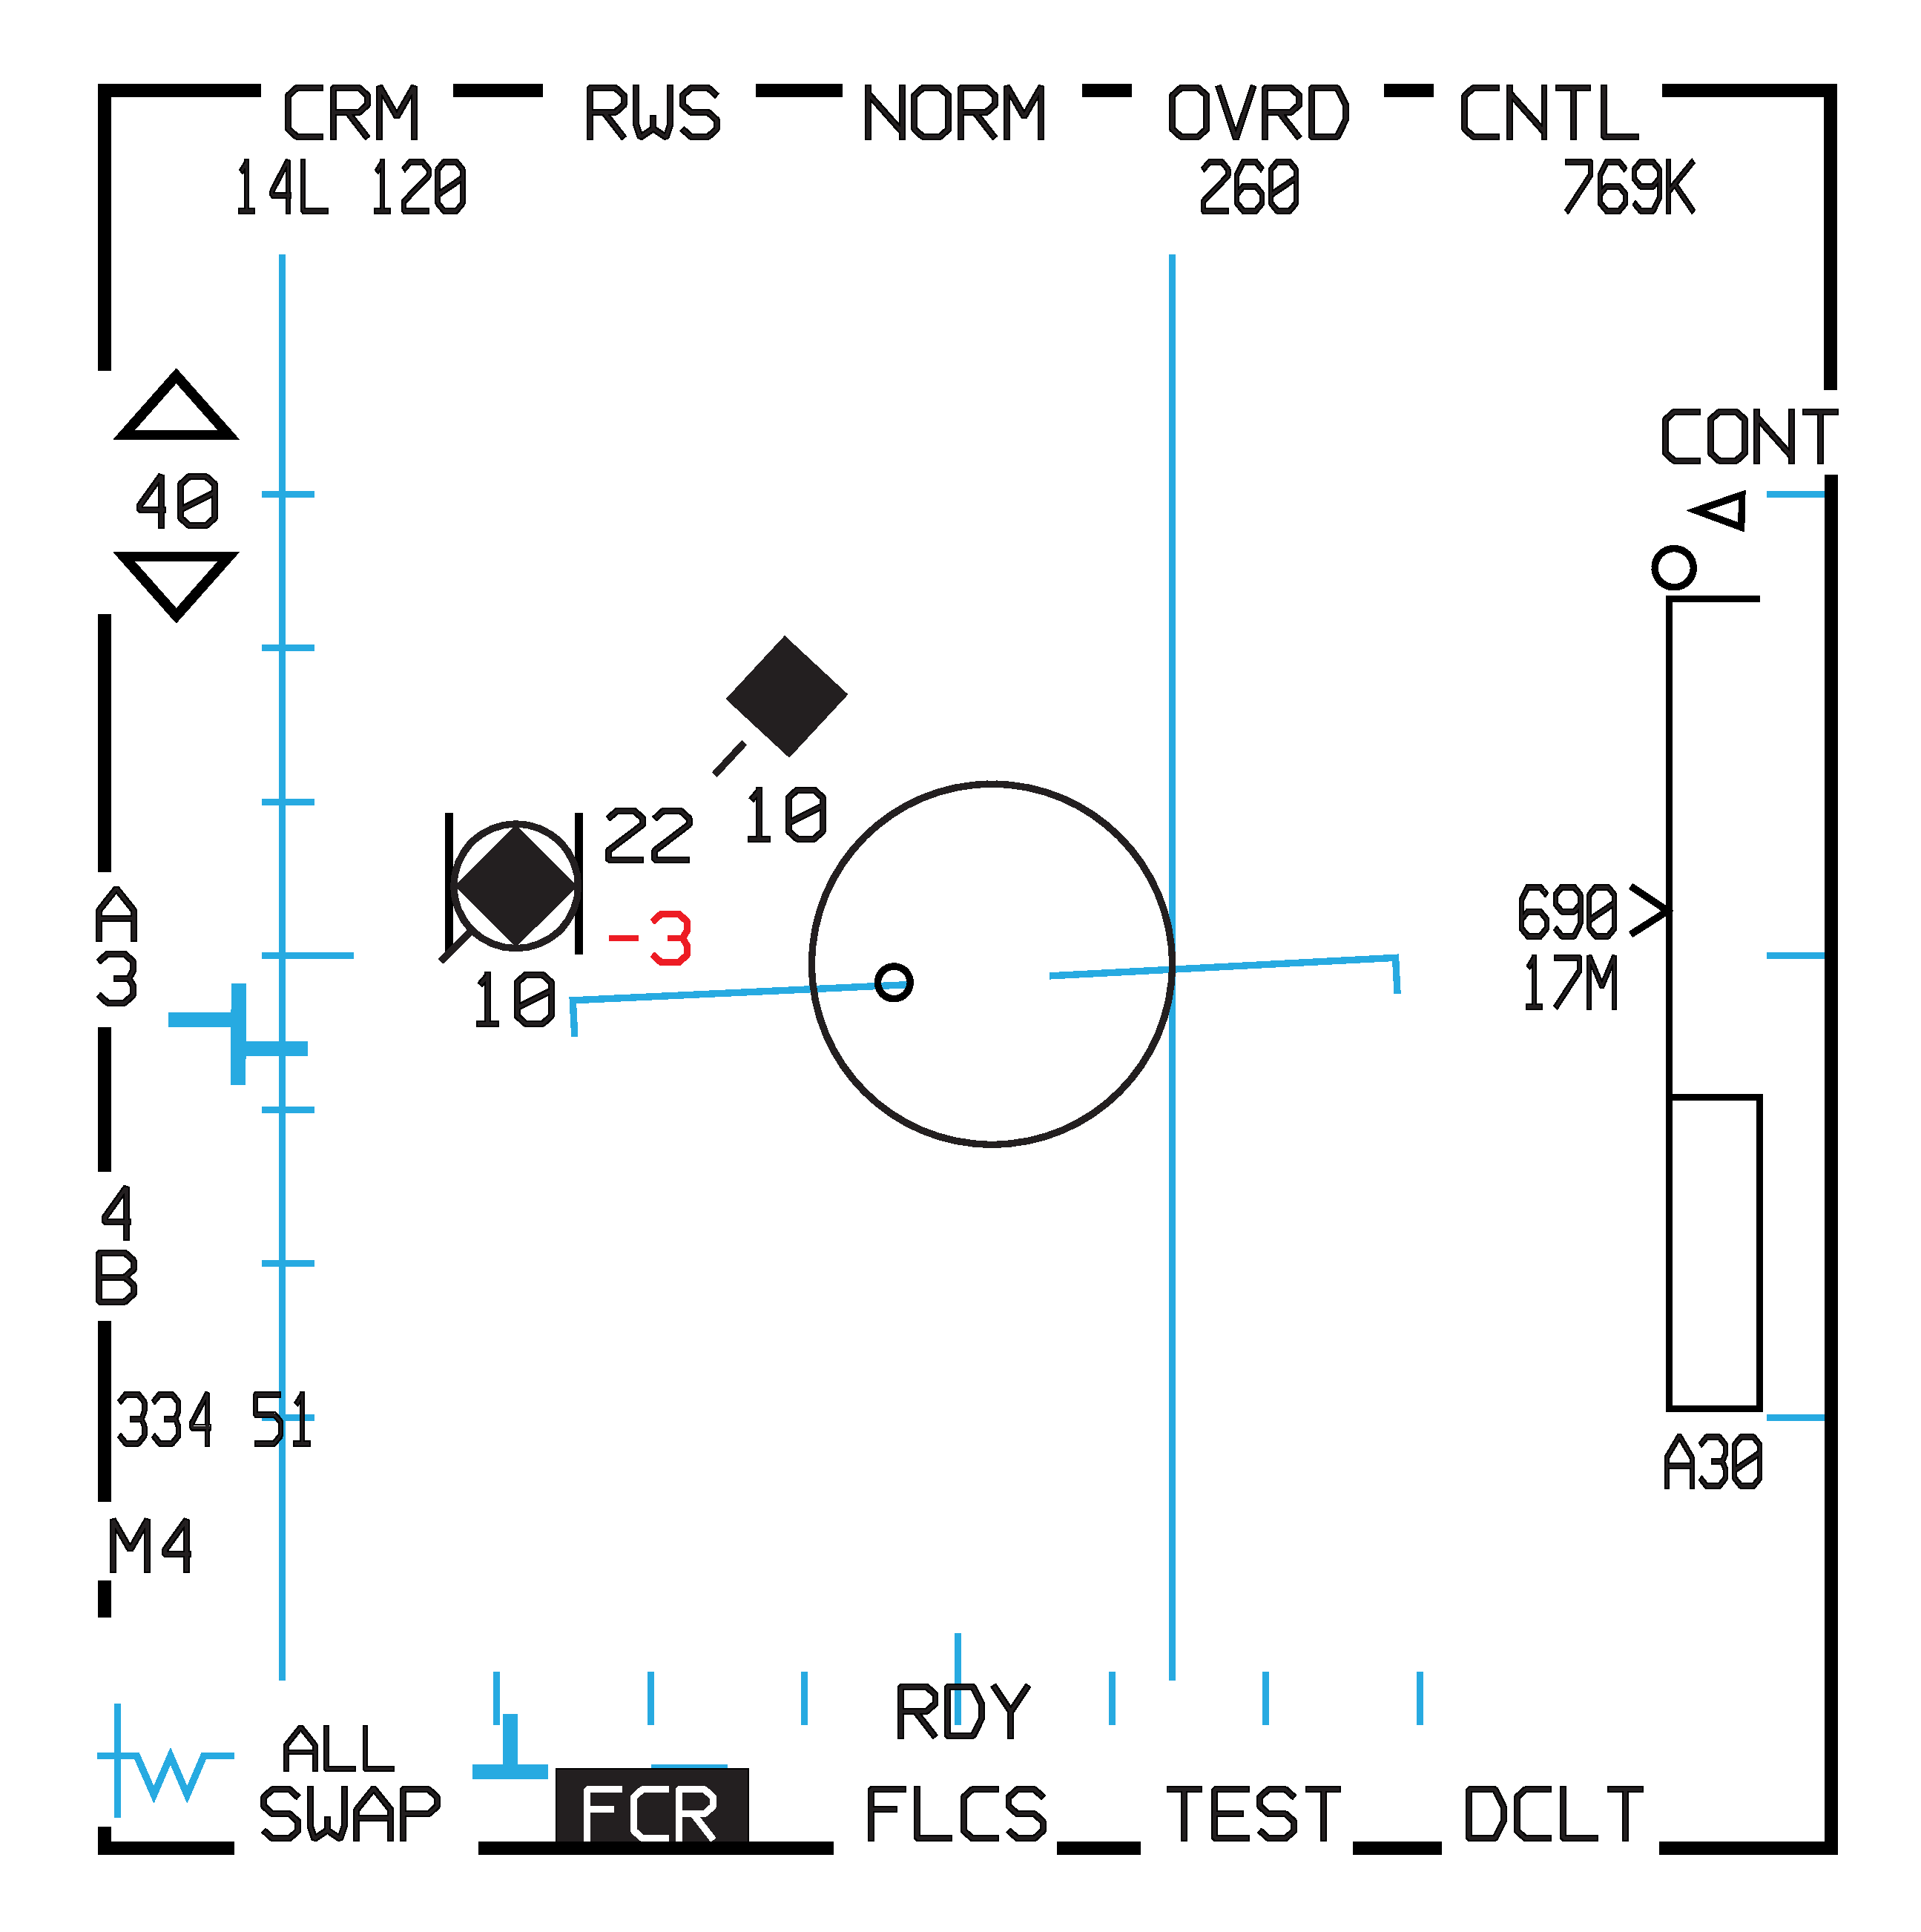
\includegraphics[
                height=75mm,
            ]{mfd/fcr_aa/rws_sam_dtt.pdf}
        };

        % Annotations
        \node[lannot] (asp) at ($(fig.west)+(0mm,30.25mm)$) {Aspect};
        \draw[annotptr] (asp.east) -- ++(9mm, 0mm);

        \node[lannot] (trk) at ($(fig.west)+(0mm,24mm)$) {Track};
        \draw[annotptr] (trk.east) -- ++(12mm, 0mm) -- ++(4mm, 4mm);

        \node[lannot] (sec) at ($(fig.west)+(0mm,10.25mm)$) {Secondary target};
        \draw[annotptr] (sec.east) -- ++(27mm, 0mm);

        \node[lannot] (prim) at ($(fig.west)+(0mm,-7mm)$) {Primary target \& cursor};
        \draw[annotptr] (prim.east) -- ++(15mm, 0mm) -- ++(4mm, 6mm);

        \node[rannot] (clos) at ($(fig.east)+(0mm,30.25mm)$) {Closure};
        \draw[annotptr] (clos.west) -- ++(-9mm, 0mm);

        \node[rannot] (as) at ($(fig.east)+(0mm,24mm)$) {Airspeed};
        \draw[annotptr] (as.west) -- ++(-22mm, 0mm) -- ++(-4mm, 4mm);

        \node[rannot] (dlz) at ($(fig.east)+(0mm,-2mm)$) {DLZ \\ {\footnotesize see \cref{fig:aa_weap:aim120:dlz}}};
        \draw[annotptr] (dlz.west) -- ++(-8mm, 0mm);

        \node[rannot] (asec) at ($(fig.east)+(0mm,-24mm)$) {ASC / ASEC \\ {\footnotesize see \cref{fig:aa_weap:aim120:asc_asec}}};
        \draw[annotptr] (asec.west) -- ++(-26mm, 0mm) -- (4mm,-7mm);

        \node[annot, anchor=south, align=left, text width=35mm] (fov) at ($(fig.north)+(-6.5mm,0mm)$) {Azimuth scan limits};
        \draw[annotptr] (fov.south) -- ++(0mm, -15mm) -- ++(12mm, -6mm);
    \end{tikzpicture}
    \caption{RWS SAM / DTT submode symbology. Additional information on primary target is displayed at top of FCR page.}
\end{figure}

\marginfigeometry

\subsubsection{SELECT RWS MODE}
\begin{checklistenumerate}
    \blueitem[FCR Switch]\dotfill \textbf{FCR}
    \blueitem[Desired MFD]\dotfill \textbf{FCR Page} verify \textbf{SOI}
    \blueitem[Radar Mode]\dotfill \textbf{CRM} (default) verify
    \begin{itemize}
        \item \textbf{Dogfight/Missile Override} --- \textbf{NORM}
        \item \textbf{Radar Mode (OSB 1)} --- shows \textbf{CRM}
    \end{itemize}
    \blueitem[CRM Submode]\dotfill \textbf{RWS} (default), 
    cycle via 
    \begin{itemize}
        \item \textbf{TMS Right (long)} / \textbf{OSB 2} 
    \end{itemize}
\end{checklistenumerate}

\subsubsection{SAM / DTT ACQUISITION}
\label{subsec:rws:samdttacq}
\begin{checklistenumerate}
    \blueitem[Locate Targets]
    \begin{enumerate}
        \item Correlate onboard/offboard sensors
        \begin{itemize}
            \item raw radar returns, RWR pings
            \item AWACS calls, datalink targets
        \end{itemize}
        \item Place targets within radar scan volume
    \end{enumerate}
    \blueitem[SAM Acquisition]
    \marginpar{
        \captionsetup{type=figure}
        \centering
        \begin{tikzpicture}[figstyle]
            
            \node[boxedmarfigstyle] (search) at (0,0) {
                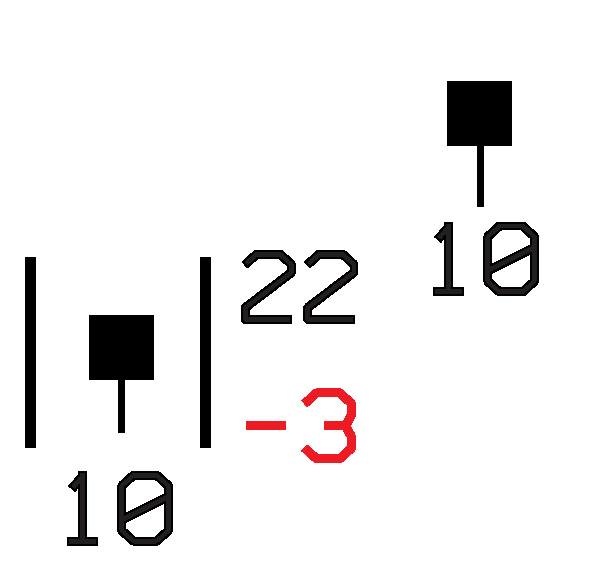
\includegraphics[
                    scale=0.25,
                ]{mfd/fcr_aa/rws_sam_dtt_subfig_01.pdf}
            };
            \node[boxedmarfigstyle] (sam) at (0,-35) {
                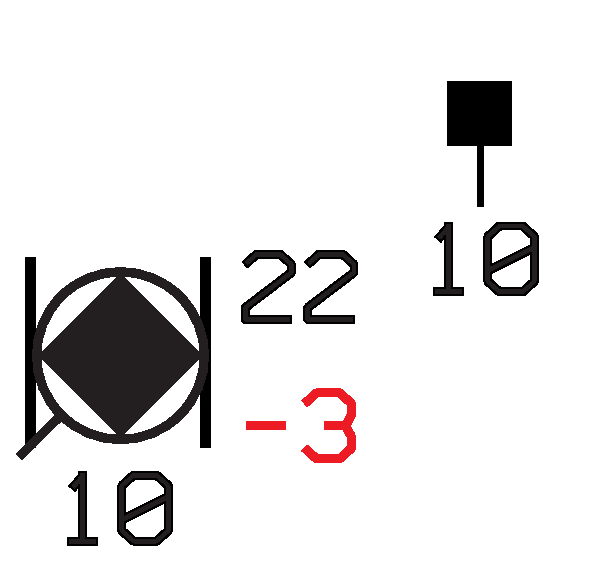
\includegraphics[
                    scale=0.25,
                ]{mfd/fcr_aa/rws_sam_dtt_subfig_02.pdf}
            };

            \draw[->]
            (search) -- node[right, align=center, font=\small] {\textbf{TMS} \textbf{FWD}}(sam);
        \end{tikzpicture}
        \caption{SAM Acquisition}
    }
    \begin{enumerate}
        \item \textbf{Target} \dotfill under Acquisition Cursor
        \item \textbf{TMS} \dotfill \textbf{Forward (hold)}
        \item \textbf{Target} \dotfill Verify \textbf{Bugged}
    \end{enumerate}
    \begin{itemize}
        \item Can guide AIM-120C on Bugged target
        \item DLZ displayed if missile selected
        \item RWS search continues
    \end{itemize}
    \blueitem[DTT Acquisition] (if desired)
    \marginpar{
        \captionsetup{type=figure}
        \centering
        \begin{tikzpicture}[figstyle]
            
            \node[boxedmarfigstyle] (sam) at (0,0) {
                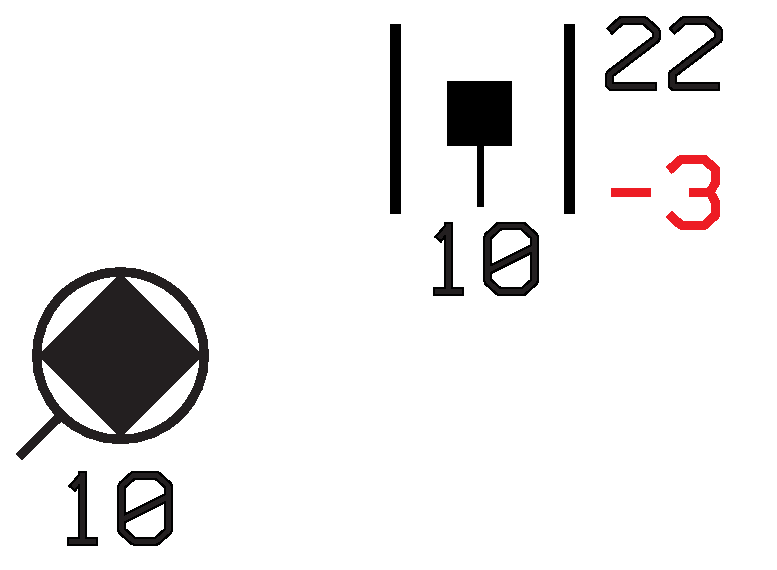
\includegraphics[
                    scale=0.25,
                ]{mfd/fcr_aa/rws_sam_dtt_subfig_03.pdf}
            };
            \node[boxedmarfigstyle] (dtt) at (0,-35) {
                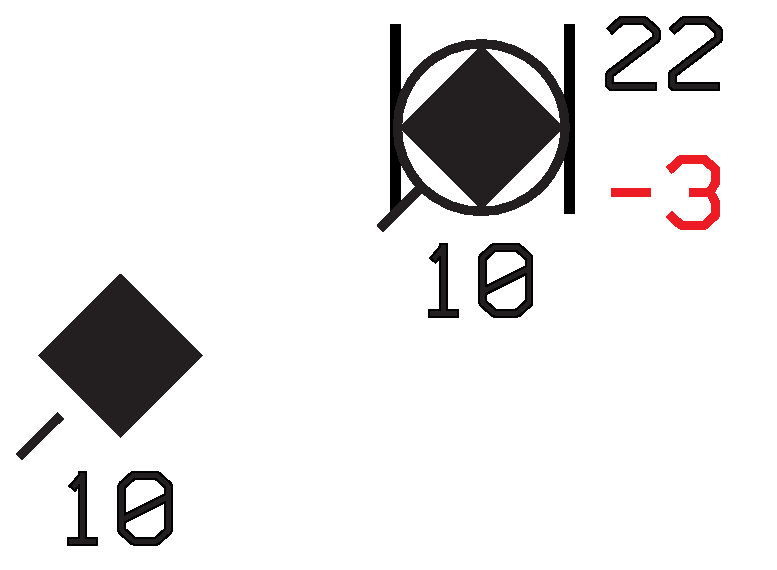
\includegraphics[
                    scale=0.25,
                ]{mfd/fcr_aa/rws_sam_dtt_subfig_04.pdf}
            };

            \draw[->]
            (sam) -- node[right, align=center, font=\small] {\textbf{TMS} \textbf{FWD}}(dtt);
        \end{tikzpicture}
        \caption{DTT Acquisition}
    }
    \begin{enumerate}
        \item \textbf{Target 2} \dotfill under Acquisition Cursor
        \item \textbf{TMS} \dotfill \textbf{Forward (hold)}
    \end{enumerate}

    To swap primary / secondary target

    \begin{enumerate}[start=3]
        \item \textbf{TMS} \dotfill \textbf{Left}
    \end{enumerate}
    \blueitem[STT Lock] (if desired)
    \begin{enumerate}
        \item \textbf{Target} \dotfill under Acquisition Cursor
        \item \textbf{TMS} \dotfill \textbf{Forward}
    \end{enumerate}
\end{checklistenumerate}

\subsubsection{SPOTLIGHT ACQUISITION}
\begin{checklistenumerate}
    \blueitem[Locate Targets]
    \begin{enumerate}
        \item Correlate onboard/offboard sensors
        \begin{itemize}
            \item raw radar returns, RWR pings
            \item AWACS calls, datalink targets
        \end{itemize}
        \item Place target within radar scan limits
    \end{enumerate}
    \blueitem[Spotlight Search]
    \marginpar{
        \captionsetup{type=figure}
        \centering
        \begin{tikzpicture}[figstyle]
            
            \node[
                boxedmarfigstyle,            
            ] (cursoroff) at (0,0) {
                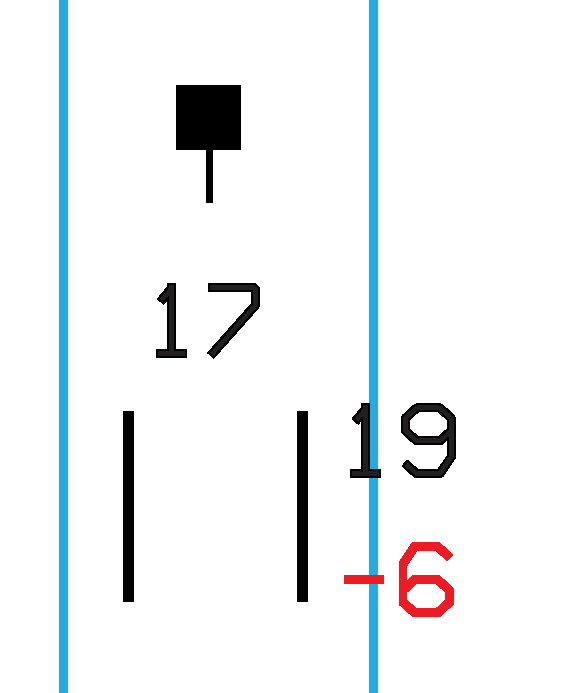
\includegraphics[
                    scale=0.25,
                ]{mfd/fcr_aa/rws_spotlight_subfig_cursor_off.pdf}
            };
            \node[
                boxedmarfigstyle,                
                below=10 of cursoroff,
            ] (cursoron) {
                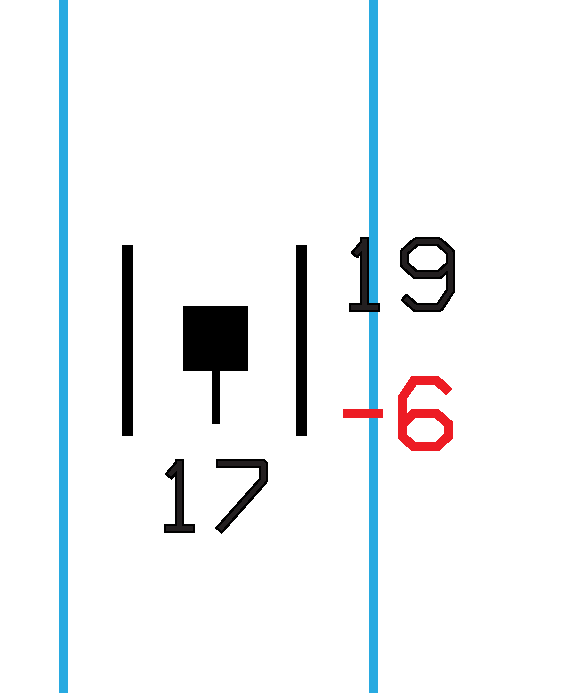
\includegraphics[
                    scale=0.25,
                ]{mfd/fcr_aa/rws_spotlight_subfig_cursor_on.pdf}
            };
            \node[
                boxedmarfigstyle,                
                below=10 of cursoron,
            ] (bugged) {
                
\includegraphics[
                    scale=0.5,
                ]{mfd/fcr_aa/tgt_bugged.pdf}
            };

            % lines
            \draw[->]
            ($(cursoroff.north) + (0,5)$) -- node[pos=0, above, align=left, font=\small] {\textbf{TMS} \textbf{FWD (hold)}}(cursoroff);
            \draw[->]
            (cursoroff) -- node[right, align=left, font=\small] {\textbf{Slew over} \\ \textbf{target}}(cursoron);
            \draw[->]
            (cursoron) -- node[right, align=left, font=\small] {\textbf{TMS FWD} \\ \textbf{(release)}}(bugged);

            % labels
            \node[
                anchor=north west,
                align=left,
                font=\bfseries\footnotesize,
            ] (labelbugged) at (bugged.north west) {Bugged \\ Target};
        \end{tikzpicture}
        \caption{Spotlight Search}
    }
    \begin{enumerate}
        \item \textbf{Target} \dotfill near Acquisition Cursor
        \item \textbf{TMS} \dotfill \textbf{Forward (hold)}
        \begin{itemize}
            \item FCR enters \pm10deg scan around acquisition cursor
        \end{itemize}
    \end{enumerate}
    \blueitem[SAM Acquisition]
    \begin{enumerate}
        \item \textbf{Target} \dotfill under Acquisition Cursor
        \item \textbf{TMS} \dotfill \textbf{Forward (release)}
        \item \textbf{Target} \dotfill Verify \textbf{Bugged}
    \end{enumerate}
    \begin{itemize}
        \item Can guide AIM-120C on Bugged target
        \item DLZ displayed if missile selected
        \item RWS search continues
    \end{itemize}
    \blueitem[STT Lock] (if desired)
    \begin{enumerate}
        \item \textbf{Target} \dotfill under Acquisition Cursor
        \item \textbf{TMS} \dotfill \textbf{Forward}
    \end{enumerate}
\end{checklistenumerate}

\marginfigrestore